\documentclass[12pt,a4paper]{article}
\usepackage[utf8]{inputenc}
\usepackage{tikz}
\usetikzlibrary{positioning,arrows.meta,shapes.gates.logic.US,calc}
\usepackage[spanish]{babel}
\usepackage[top=2.5cm, bottom=2.5cm, left=3cm, right=3cm]{geometry}
\usepackage{setspace}
\onehalfspacing
\usepackage{graphicx}
\usepackage{fancyhdr}
\usepackage{enumitem}
\usepackage{booktabs}
\usepackage{hyperref}
\hypersetup{hidelinks}
\usepackage{tabularx}
\usepackage{amssymb}
\usepackage{amsmath}
\usepackage{listings}
\usepackage{xcolor}

\setlength{\headheight}{14.5pt}

\pagestyle{fancy}
\fancyhf{}
\lhead{\textit{Arquitectura de Computadoras}}
\rhead{\textit{Práctica 07 -- Multiplexor 4$\times$1 con lógica}}
\cfoot{\thepage}
\renewcommand{\headrulewidth}{0.4pt}

\makeatletter
\renewcommand{\@seccntformat}[1]{\csname the#1\endcsname.\quad}
\makeatother

\setlist[itemize]{label=\footnotesize$\blacksquare$, itemsep=0.15\baselineskip, topsep=0.5\baselineskip}
\setlist[enumerate]{label=\alph*), itemsep=0.15\baselineskip, topsep=0.5\baselineskip}

\definecolor{codebg}{RGB}{248,248,248}
\definecolor{codekey}{RGB}{0,90,160}
\definecolor{codecom}{RGB}{120,120,120}
\lstdefinelanguage{VHDL}{
  morekeywords={library,use,all,entity,is,port,in,out,end,architecture,of,
    begin,signal,process,if,then,else,elsif,case,when,others,with,select,
    not,and,or,nand,nor,xor,to,for,loop,wait,report,severity,error,failure,
    variable,constant,type,array,downto,std_logic,std_logic_vector,integer},
  sensitive=true,
  morecomment=[l]{--}
}
\lstset{
  language=VHDL,
  basicstyle=\ttfamily\footnotesize,
  keywordstyle=\color{codekey}\bfseries,
  commentstyle=\color{codecom}\itshape,
  backgroundcolor=\color{codebg},
  frame=single,
  rulecolor=\color{black!30},
  breaklines=true,
  showstringspaces=false,
  columns=fullflexible,
  xleftmargin=0.5em,
}

\title{}
\author{}

\begin{document}

% ==========================================
% PORTADA
% ==========================================
\begin{titlepage}
    \centering
    \vspace*{1cm}
    {\Large\bfseries Universidad Autónoma de Zacatecas\par}
    \vspace{0.4cm}
    {\large\bfseries Unidad Académica de Ingeniería Eléctrica\par}
    {\large\bfseries Ing. Electrónica Industrial con Esp. en Telecomunicaciones\par}
    \vspace{1.5cm}
    \noindent\rule{\textwidth}{0.8pt}
    \vspace{1cm}
    {\huge\bfseries Práctica 07\par}
    \vspace{0.7cm}
    {\Large ``Multiplexor 4$\times$1 con lógica combinatoria \\ en cada canal''\par}
    \vspace{1cm}
    \noindent\rule{\textwidth}{0.8pt}
    \vspace{1.8cm}

    \begin{tabular}{r l}
        \textbf{Materia:}    & Arquitectura de Computadoras \\[0.35cm]
        \textbf{Práctica:}   & Práctica 07 \\[0.35cm]
        \textbf{Alumno(a):}  & Arnold Yovick Rios Zaldivar \\[0.35cm]
        \textbf{Matrícula:}  & 35167151 \\[0.35cm]
        \textbf{Docente:}    & Angel García Durán \\[0.35cm]
        \textbf{Fecha:}      & 25 de septiembre de 2026
    \end{tabular}

    \vfill
    Ciclo escolar: Ago--Dic 2026
    \vspace*{0.5cm}
\end{titlepage}
\setcounter{page}{1}

% ==========================================
% INTRODUCCIÓN
% ==========================================
\section{Introducción}

En los sistemas digitales es frecuente que varias señales compartan un mismo
medio de salida, ya sea un bus de datos, un puerto o la entrada de un bloque
posterior. Para decidir cuál de esas señales llega en cada instante puede
utilizarse un \textbf{multiplexor}, un circuito combinatorio que selecciona una
de $2^n$ entradas de datos y la entrega a una única salida, en función de $n$
líneas de selección. El multiplexor es, en esencia, el opuesto del
demultiplexor que se trabajó en una práctica previa: mientras el demux
``reparte'' un dato hacia varias vías, el mux ``recolecta'' el dato de una de
varias vías.

En esta práctica se propone un circuito que combina ambas ideas: un
\textbf{multiplexor 4$\times$1} cuyas entradas de datos no son señales
directas, sino el resultado de \textbf{bloques de lógica combinatoria}
construidos con compuertas AND, OR, NOT, NAND y NOR. El problema consta de
nueve entradas ($ent(0)$ a $ent(8)$), dos líneas de selección ($s(1)$ y $s(0)$)
y una salida única ($sal$). Cada uno de los cuatro canales del multiplexor
calcula una función distinta a partir de un subconjunto de las entradas, y la
línea de selección determina cuál de esas cuatro funciones aparece en la
salida.

El objetivo de la práctica es, por un lado, \textbf{traducir un diagrama
esquemático de compuertas a código VHDL} y, por otro, \textbf{verificar
mediante simulación} que la implementación coincide con la función descrita por
dicho diagrama. Como herramienta se utiliza \textbf{GHDL} para la compilación y
simulación, y \textbf{GTKWave} para la inspección de las formas de onda. Se
adoptó además un enfoque de \emph{autoverificación} mediante \texttt{assert},
vigente en prácticas anteriores, que permite confirmar el diseño sin depender
de la lectura manual de las ondas.

% ==========================================
% MATERIALES Y MÉTODOS
% ==========================================
\section{Materiales y métodos}

\subsection*{Materiales}

\begin{itemize}
    \item Entorno GNU/Linux con la cadena de herramientas \textbf{GHDL}
          (analizador, elaborador y simulador de VHDL).
    \item \textbf{GTKWave} como visor de formas de onda (\texttt{.vcd}).
    \item El diagrama esquemático de referencia proporcionado en la clase,
          que define las compuertas de cada canal y el multiplexor 4$\times$1.
    \item Un archivo fuente \texttt{circuito.vhd} con la
          \texttt{entity}/\texttt{architecture} del diseño y un archivo
          \texttt{tb\_circuito.vhd} con el banco de pruebas.
\end{itemize}

\subsection*{Método}

El flujo de trabajo sigue el ciclo habitual de la materia: \emph{escribir el
diseño} $\rightarrow$ \emph{escribir el banco de pruebas} $\rightarrow$
\emph{compilar y simular} $\rightarrow$ \emph{inspeccionar las ondas}. Los pasos
concretos fueron:

\begin{enumerate}
    \item \textbf{Lectura del diagrama.} Se identificaron las compuertas de
          cada canal y se derivó su expresión booleana:
          \begin{align}
            c_0 &= \overline{ent(0)} + ent(1), \label{eq:c0}\\
            c_1 &= \overline{\overline{ent(2) + ent(3) + ent(4)} \cdot ent(5)}, \label{eq:c1}\\
            c_2 &= ent(5)\,ent(6) + ent(7)\,ent(8), \label{eq:c2}\\
            c_3 &= ent(5)\,ent(6)\,ent(7) \oplus ent(8). \label{eq:c3}
          \end{align}
          Nótese que $c_1$ es una NAND de 2 entradas cuyo primer término es la
          NOR de \texttt{ent(2)}, \texttt{ent(3)} y \texttt{ent(4)}, y que
          $c_3$ es una XOR entre la AND de tres entradas
          \texttt{ent(5)},\texttt{ent(6)},\texttt{ent(7)} y \texttt{ent(8)}.
    \item \textbf{Codificación del diseño.} Se escribieron dos arquitecturas
          equivalentes: una \emph{estructural}, que nombra cada compuerta
          intermedia mediante señales y reproduce el diagrama paso a paso, y
          una \emph{simplificada}, que condensa cada canal en una sola
          expresión. La selección se implementó con la estructura
          \texttt{with~/~select}, ya conocida de prácticas anteriores.
    \item \textbf{Banco de pruebas autoverificado.} El \texttt{testbench}
          recorre las cuatro posiciones del selector y las $2^9 = 512$
          combinaciones de las nueve entradas (2048 casos en total). Para cada
          caso calcula un valor esperado con las expresiones
          \eqref{eq:c0}--\eqref{eq:c3} y lo compara
          contra las salidas de \emph{ambas} arquitecturas mediante
          \texttt{assert}. Si algún caso no coincide, la simulación falla con
          \texttt{severity failure}.
    \item \textbf{Compilación y ejecución.}
\begin{lstlisting}[language=bash]
ghdl -a circuito.vhd tb_circuito.vhd   # analiza
ghdl -e tb_circuito                    # elabora
ghdl -r tb_circuito --vcd=tb_circuito.vcd   # simula y graba ondas
\end{lstlisting}
    \item \textbf{Inspección.} El archivo \texttt{tb\_circuito.vcd} se abre en
          GTKWave para observar el comportamiento del selector y confirmar
          visualmente los resultados.
\end{enumerate}

% ==========================================
% RESULTADOS
% ==========================================
\section{Resultados}

\subsection*{Circuito implementado}

La Figura~\ref{fig:circuito} muestra el diagrama del circuito implementado,
con las cuatro ramas de lógica combinatoria alimentando las entradas del
multiplexor 4$\times$1 controlado por $s(1)\,s(0)$.

\begin{figure}[h]
    \centering
    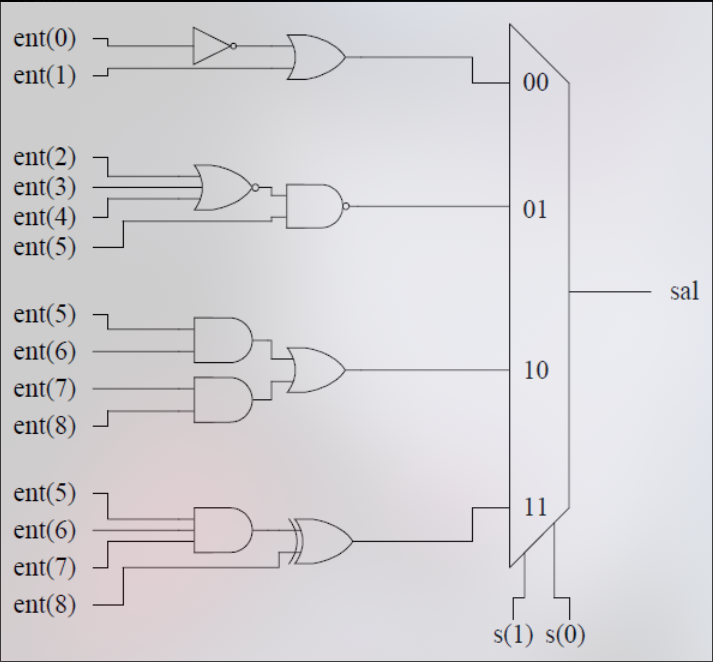
\includegraphics[width=0.92\textwidth]{circuito.png}
    \caption{Diagrama del multiplexor 4$\times$1 con lógica combinatoria en
    cada canal, proporcionado en clase. Cada rama calcula una de las
    funciones $c_0$--$c_3$ y el selector $s(1)\,s(0)$ elige cuál llega a la
    salida.}
    \label{fig:circuito}
\end{figure}

\subsection*{Verificación por simulación}

La simulación terminó sin errores y con el siguiente mensaje, que resume la
autoverificación de los 2048 casos:

\begin{lstlisting}[language=bash]
tb_circuito.vhd:68:5:@2048ns:(report note):
OK: 4 selectores x 512 combinaciones = 2048 casos correctos.
\end{lstlisting}

Esto significa que, para \emph{todas} las combinaciones de las nueve entradas y
las cuatro posiciones del selector, la arquitectura estructural, la
simplificada y el modelo de referencia coincidieron entre sí.

\subsection*{Tabla de comportamiento por canal}

La Tabla~\ref{tab:canales} resume la función que selecciona cada valor de $s$
y algunos casos representativos.

\begin{table}[h]
    \centering
    \begin{tabular}{@{}cccl@{}}
        \toprule
        $s(1)$ & $s(0)$ & Función en $sal$ & Ejemplo \\
        \midrule
        0 & 0 & $c_0 = \overline{ent(0)} + ent(1)$ & $ent(0)=0,ent(1)=0 \Rightarrow 1$ \\
        0 & 1 & $c_1 = \overline{\overline{ent(2)+ent(3)+ent(4)}\,ent(5)}$ & $ent(2..4)=000 \Rightarrow 1$ \\
        1 & 0 & $c_2 = ent(5)\,ent(6) + ent(7)\,ent(8)$ & $ent(5)=ent(6)=1 \Rightarrow 1$ \\
        1 & 1 & $c_3 = ent(5)\,ent(6)\,ent(7) \oplus ent(8)$ & $ent(5..7)=111,\,ent(8)=0 \Rightarrow 1$ \\
        \bottomrule
    \end{tabular}
    \caption{Comportamiento del multiplexor según el selector.}
    \label{tab:canales}
\end{table}

\subsection*{Forma de onda}

La Figura~\ref{fig:onda} muestra la forma de onda obtenida en GTKWave. El
selector $s(1)\,s(0)$ avanza en cuatro tramos ($00 \to 01 \to 10 \to 11$),
mientras las nueve entradas recorren sus combinaciones. Se aprecia que la
salida de la arquitectura estructural (\texttt{sal\_est}) y la de la
simplificada (\texttt{sal\_sim}) son idénticas en todo instante, y que
\texttt{sal} reproduce en cada tramo la función del canal habilitado: $c_0$
(densa, por depender de los bits menos significativos), $c_1$ (casi siempre en
alto, con caídas cuando $ent(4\ldots2)=000$ y $ent(5)=1$), $c_2$ y $c_3$
(pulsos espaciados, por depender de los bits más significativos). Las señales
internas \texttt{n0}, \texttt{nor234}, \texttt{a56}, \texttt{a78} y
\texttt{a567} evidencian cada compuerta intermedia del diagrama.

\begin{figure}[h]
    \centering
    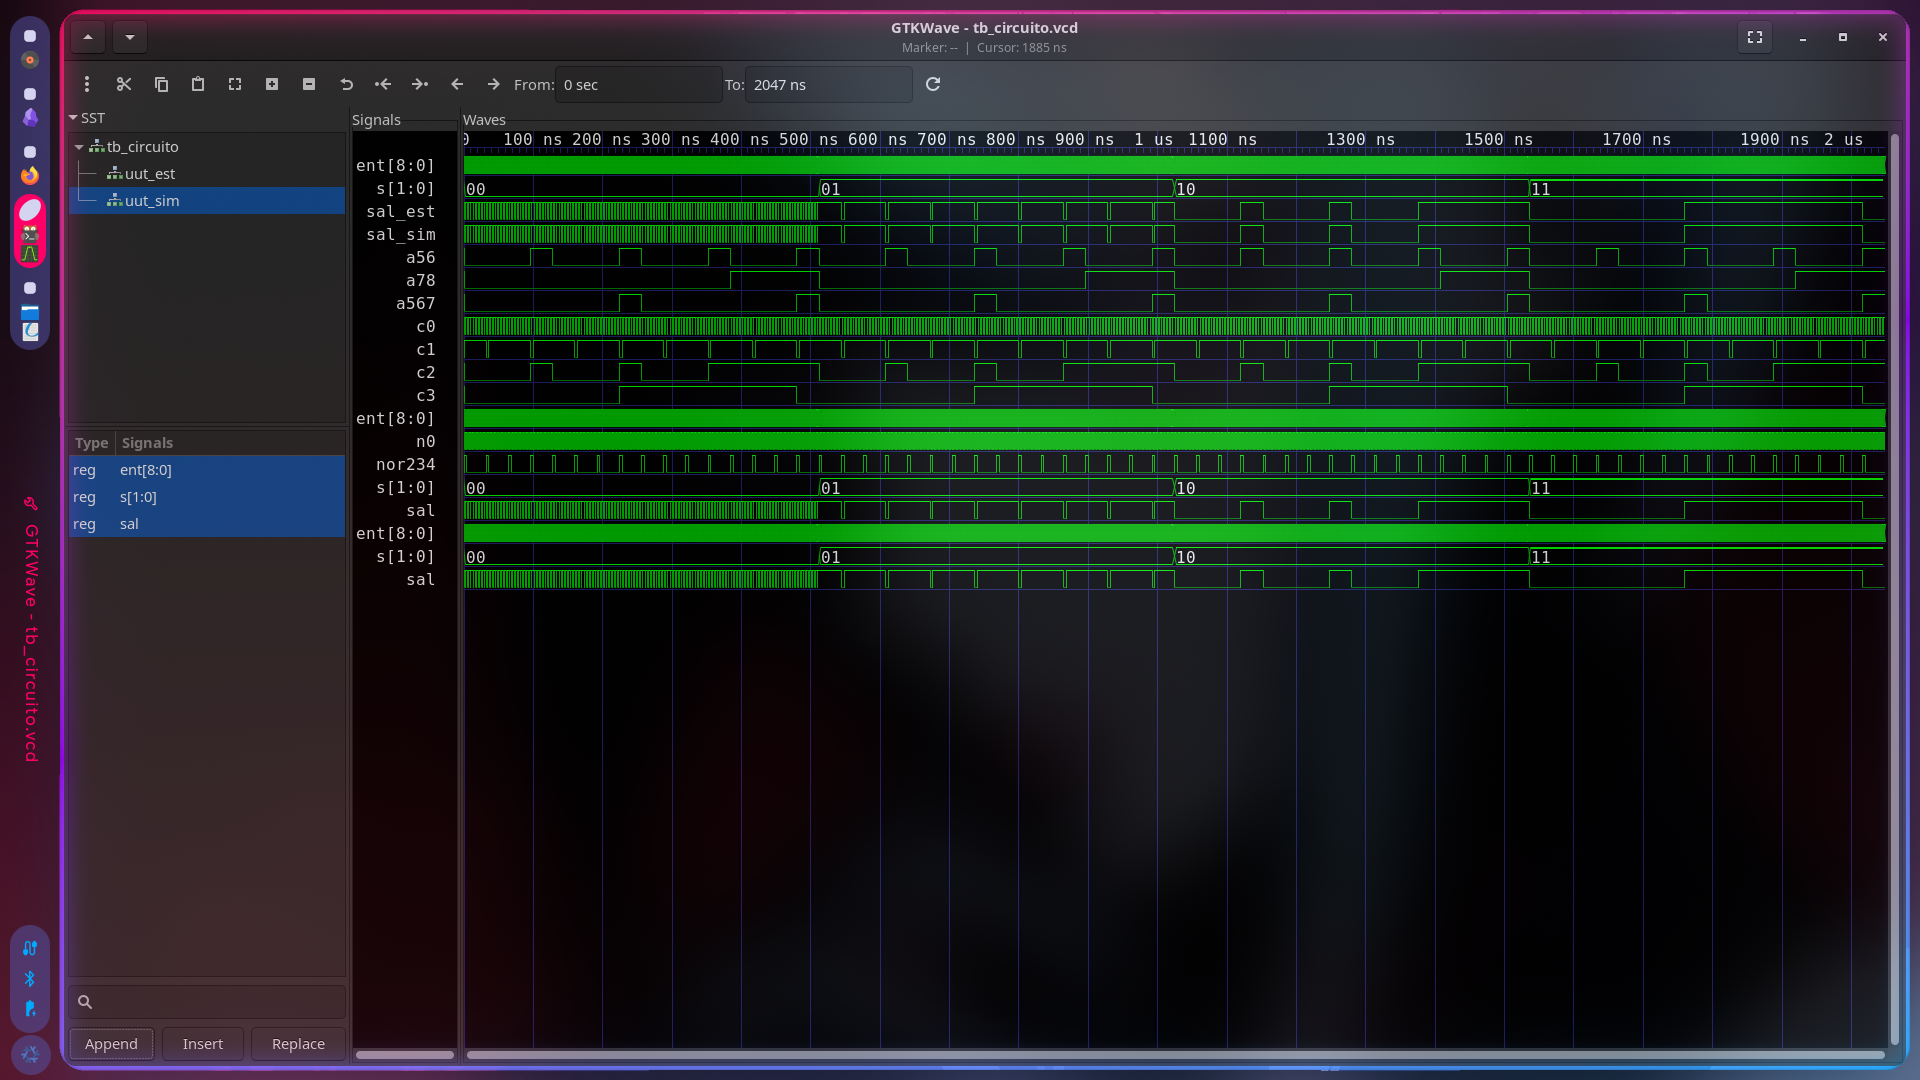
\includegraphics[width=\textwidth]{gtkwave.png}
    \caption{Simulaci\'on del circuito corregido en GTKWave. El selector
    $s(1)\,s(0)$ recorre $00,01,10,11$; las se\~nales \texttt{sal\_est} y
    \texttt{sal\_sim} (arquitecturas estructural y simplificada) coinciden en
    todo instante, y \texttt{sal} reproduce el canal habilitado
    ($c_0$--$c_3$).}
    \label{fig:onda}
\end{figure}

% ==========================================
% CONCLUSIONES
% ==========================================
\section{Conclusiones}

La práctica permitió integrar dos bloques ya vistos por separado: la lógica
combinatoria con compuertas y el multiplexor como elemento de selección. Se
comprobó que un multiplexor 4$\times$1 puede alimentarse con funciones
booleanas arbitrarias y que la línea de selección decide cuál de ellas llega a
la salida, lo que ilustra de forma directa el concepto de \emph{selección de
datos} en los sistemas digitales. El paso del diagrama esquemático a VHDL fue
sencillo una vez establecidas las expresiones de cada canal
\eqref{eq:c0}--\eqref{eq:c3}, y la estructura \texttt{with~/~select} resultó
idónea para modelar el multiplexor.

El resultado más valioso fue la estrategia de \emph{autoverificación}: en lugar
de confiar en la inspección visual de las ondas, el banco de pruebas comparó
automáticamente las 2048 combinaciones contra un modelo de referencia y
verificó además que ambas arquitecturas (estructural y simplificada) coinciden.
Esto reduce el riesgo de errores de lectura y hace que el diseño sea
reutilizable y confiable. Finalmente, el contraste entre la versión
compuerta por compuerta y la versión condensada en una expresión muestra que,
en VHDL, la descripción estructural y la descripción por comportamiento son
equivalentes en función aunque difieran en legibilidad y en cercanía al
diagrama original.

% ==========================================
% BIBLIOGRAFÍA
% ==========================================
\begin{thebibliography}{9}
    \bibitem{ghdl}
    T. Gingold, \textit{GHDL: VHDL simulator}, documentación oficial.
    [En línea]. Disponible en: \url{https://ghdl.github.io/ghdl/}

    \bibitem{gtkwave}
    A. Bybell, \textit{GTKWave: waveform viewer}, documentación oficial.
    [En línea]. Disponible en: \url{https://gtkwave.sourceforge.net/}

    \bibitem{ieee1076}
    IEEE, \textit{IEEE Standard VHDL Language Reference Manual},
    IEEE Std 1076, 2019.
\end{thebibliography}

\end{document}
